\section{Pianificazione}
Alla luce delle scadenze presentate nella \hyperlink{scadenze}{sottosezione 2.5} la pianificazione di progetto viene suddivisa nelle seguenti fasi:
\begin{enumerate}
	\item \textbf{Analisi};
	\item \textbf{Consolidamento dei Requisiti};
	\item \textbf{Progettazione Architetturale}
	\item \textbf{text}
\end{enumerate}
Ogni fase viene suddivisa in attività\glosp che verranno realizzate durante il 
periodo stabilito per la fase stessa. 
\subsection{Analisi}
\textit{Periodo: dal 2018-11-16 al 2019-01-14}\\
L'inizio del periodo di questa fase coincide con la data di formazione dei 
gruppo e la fine coincide con la data di consegna dei documenti relativi alla 
revisione dei requisiti. Questa fase è stata scomposta nelle seguenti attività:
\begin{itemize}
	\item \textbf{Individuazione degli strumenti}: questa attività consiste nel 
	determinare quali strumenti il gruppo deve utilizzare per la comunicazione 
	e per la stesura dei documenti; 
	\item \textbf{Norme di Progetto}: sono definite tutte le regole utili per lo svolgimento del progetto, relative al prodotto da realizzare e ai processi da adottare. ;iene redatto il documento \textit{Norme 
	di Progetto}, che formalizza le norme sopracitate, dal responsabile di progetto e dall'amministratore;
	\item \textbf{Studio di fattibilità}: in questa attività i membri del gruppo effettuano uno studio sommario dei capitolati in modo da determinare quale di essi verrà scelto. Inoltre viene redatto il documento 
	\textit{Studio di fattibilità} nel quale vengono riportate le considerazioni del gruppo sui i capitolati proposti e viene indicato il capitolato scelto dal gruppo. 
	Questa attività e da considerarsi bloccante per l'attività di Analisi dei 
	Requisiti;
	\item \textbf{Analisi dei Requisiti}: durante questa attività vengono 
	identificati ed analizzati i requisiti del capitolato scelto nell'attività 
	precendente e viene redatto di conseguenza il documento \textit{Analisi dei 
	Requisiti};
	\item \textbf{Piano di Progetto}: viene pianificato il 
	lavoro del gruppo 8Lab Solutions, inteso come suddivisione di compiti, 
	risorse e attività. Inoltre si prospetta il preventivo per la realizzazione 
	del progetto. Questa attività comporta anche la stesura 
	del documento \textit{Piano di Progetto};
	\item \textbf{Piano di Qualifica}: in questà attività si individuano le 
	metodologie attraverso le quali si garatisce la qualità del prodotto. A supporto di ciò viene redatto il documento \textit{Piano di Qualifica}; 
	\item \textbf{Glossario}: vengono individuati tutti i termini poco chiari e 
	vengono disambiguati nel documento \textit{Glossario} il quale viene 
	redatto durante tutta la fase di analisi dei requisiti.
\end{itemize}
\subsubsection{Diagramma di Gantt}
\begin{figure}[H]
	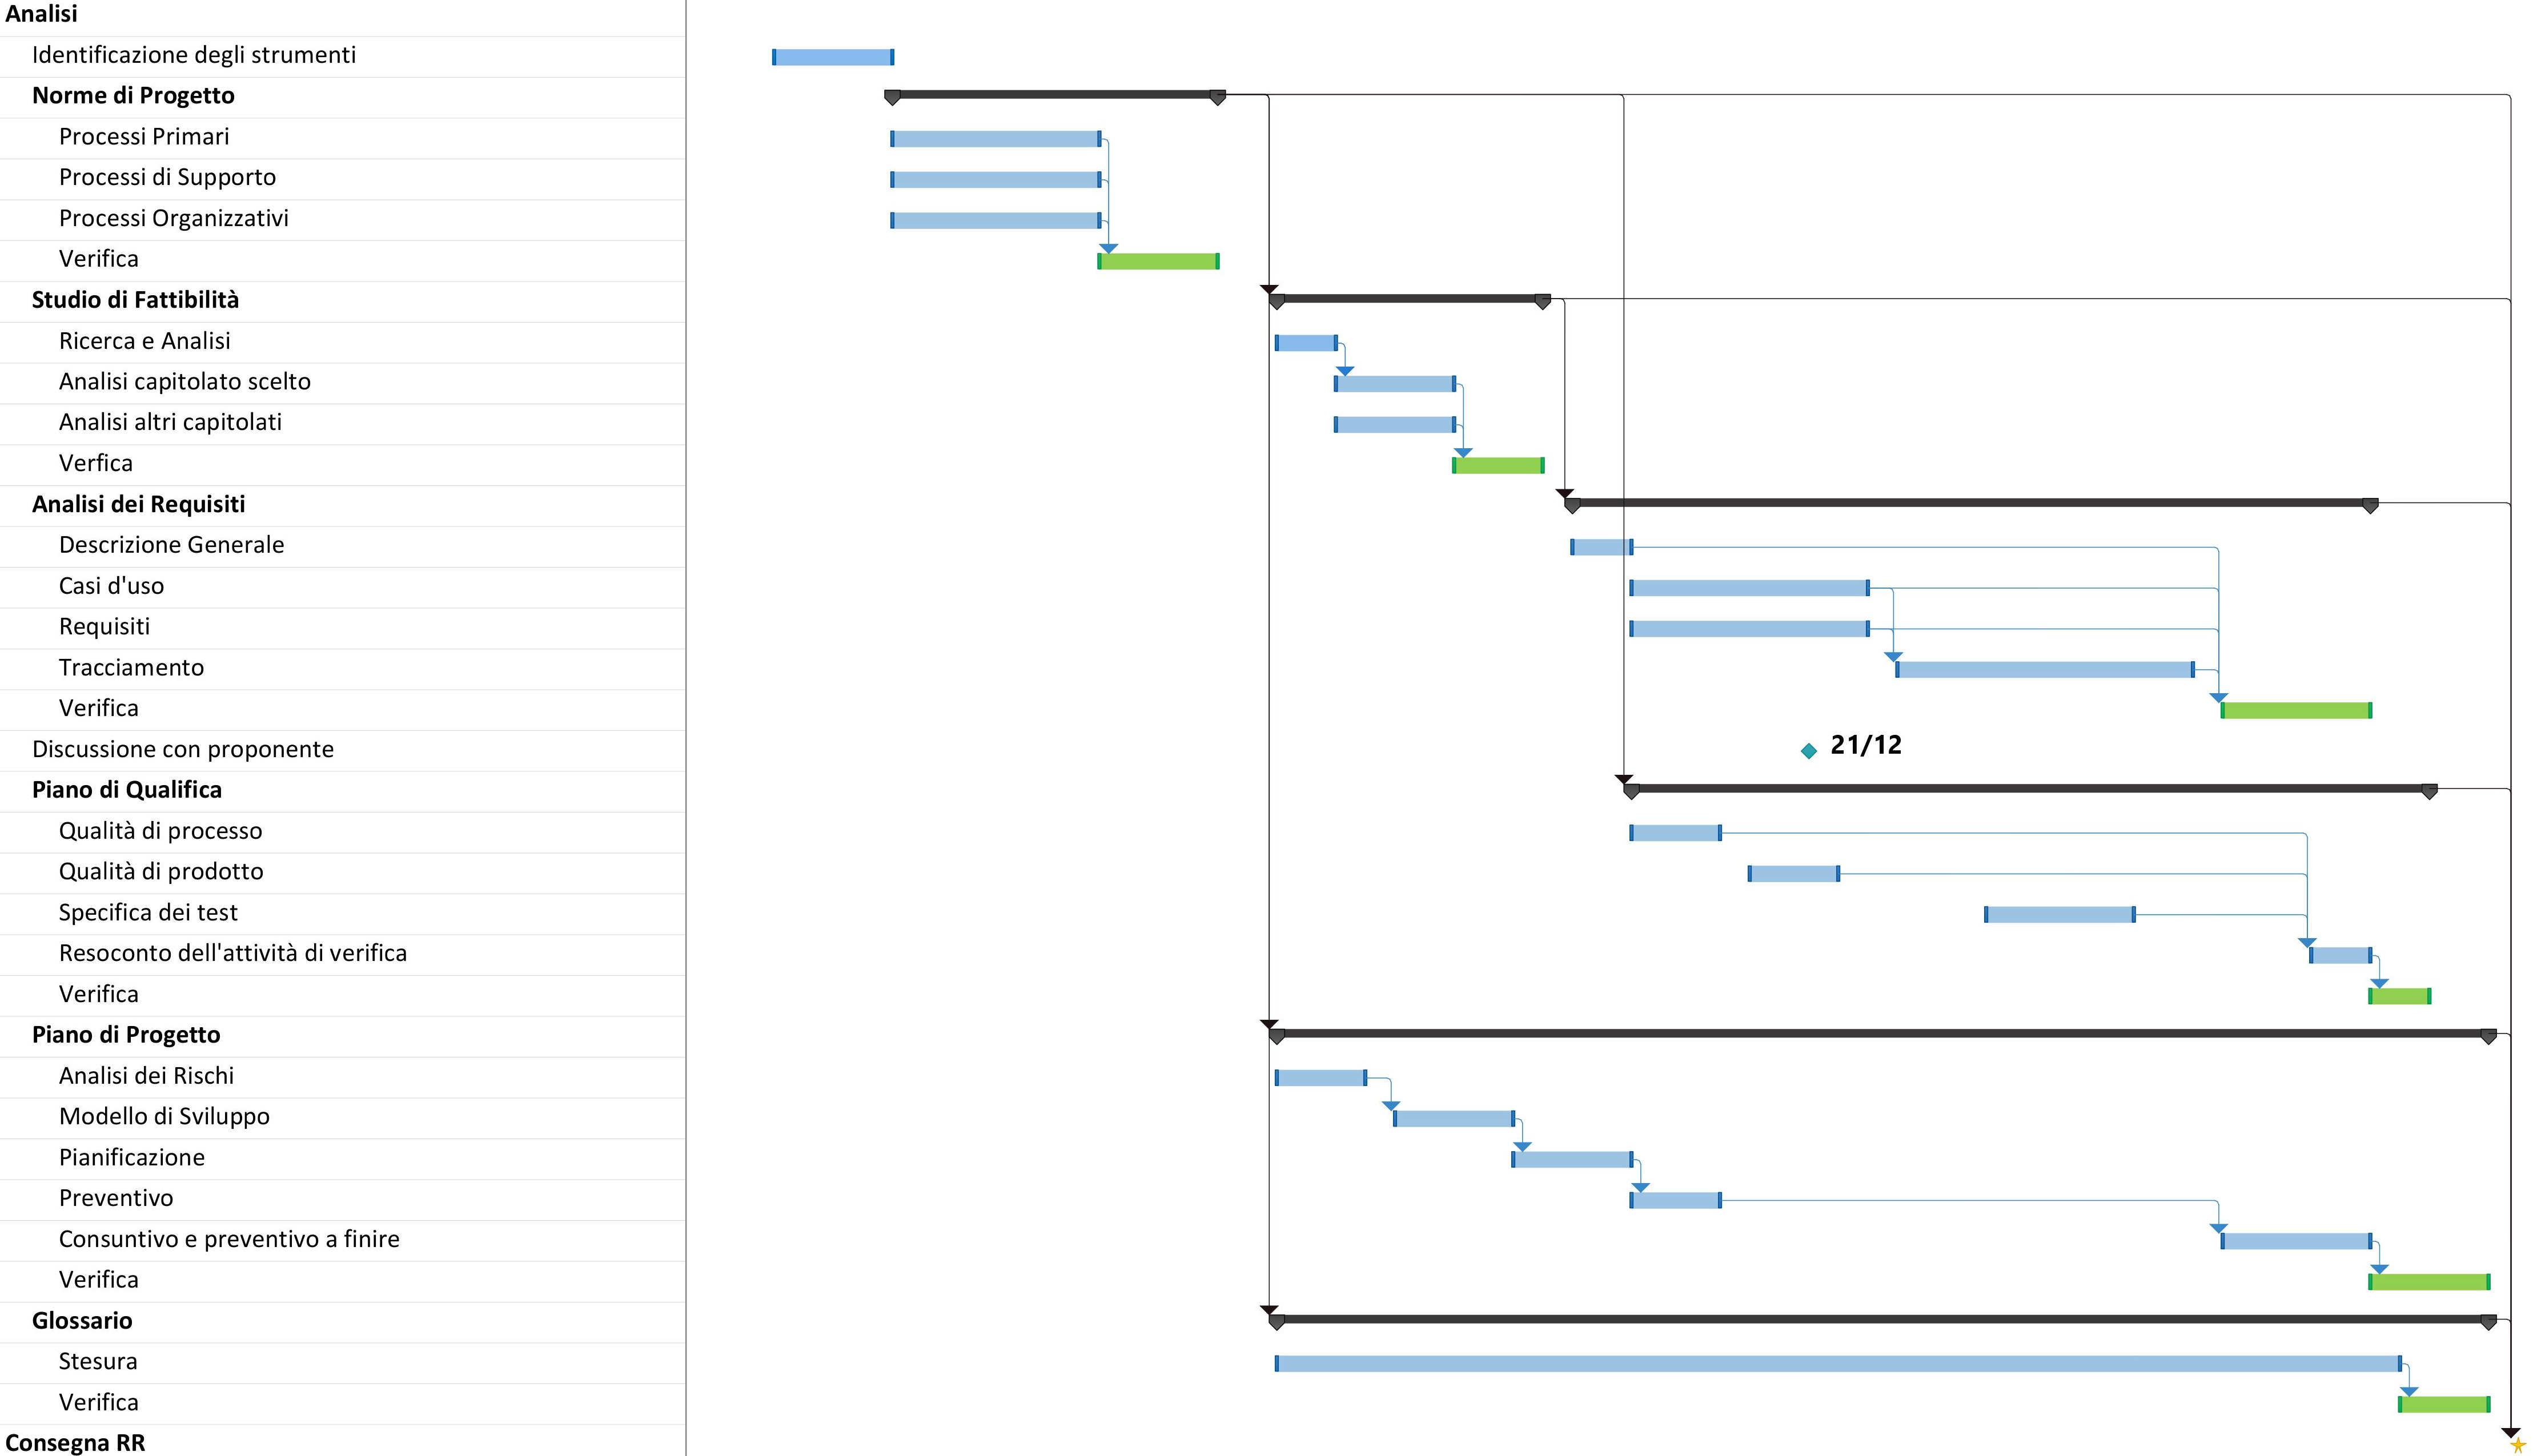
\includegraphics[scale=0.8]{res/images/gantt_analisi.jpg}
	\caption{Diagramma di Gantt della prima fase}
\end{figure}
\pagebreak
\subsection{Consolidamento dei Requisiti}
\textit{Perdiodo: dal 2019-01-14 al 2019-01-21} \\
Questa fase comincia con la fine della fase di \textit{Analisi} e termina il giorno della presentazione della \textit{Revisione dei Requisiti}. Le attività di questa fase sono:
\begin{itemize}
	\item \textbf{Consolidamento}: questa attività ha lo scopo di consolidare e migliorare i requisiti ottenuti nella fase precendente;
	\item \textbf{Incremento e Verifica}: se necessario vengono migliorati i documenti prodotti nella fase precendente.
\end{itemize}

\begin{figure}[H]
	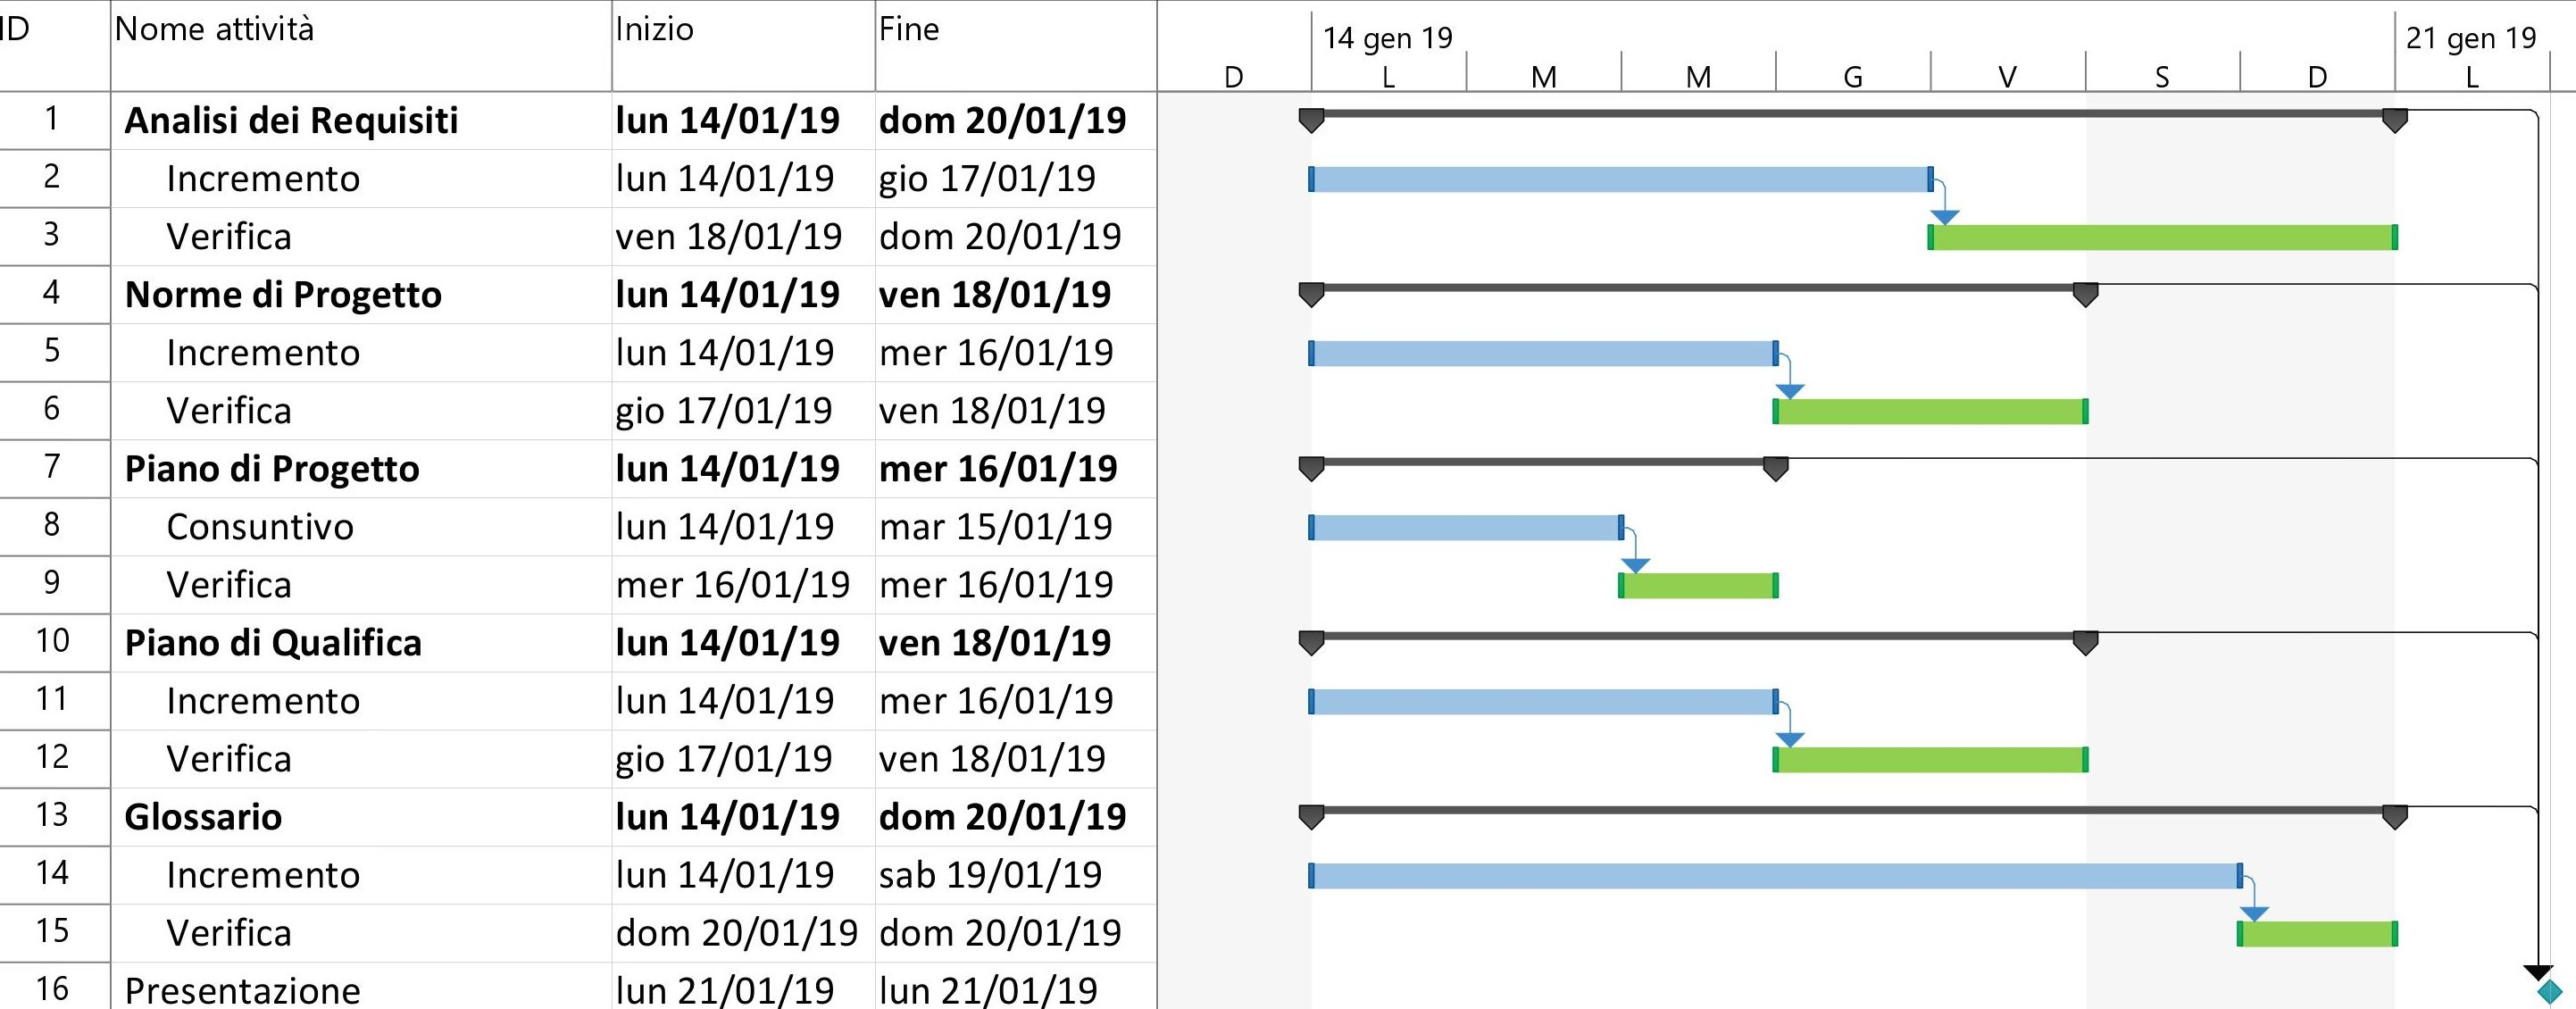
\includegraphics[scale=0.6]{res/images/gantt_cons.jpg}
	\caption{Diagramma di Gantt della prima fase}
\end{figure}
\pagebreak
\subsection{Progettazione Architetturale}